\providecommand{\main}{../../..}
\documentclass[\main/main.tex]{subfiles}
\begin{document}

\subsection{Esercizio 6}
Si consideri un problema di teoria delle decisioni con 3 soluzioni alternative, indicate da $x_1$, $x_2$ e $x_3$ e 2 stati di natura, indicati da $\omega_1$ e $\omega_2$.

Le seguenti tabelle riportano la funzione $f(x, \omega)$ che rappresenta dei benefici e le probabilità congiunte $p(\omega, y)$ degli stati di natura e dei risultati di un esperimento che può avere 2 esiti, indicati da $y_1$ e $y_2$. Qual è la strategia ottima?

\begin{figure}
  \begin{subfigure}{0.49\textwidth}
    \begin{table}
      \begin{tabular}{|L|L|L|}
        \hline
        f(x, \omega) & \omega_1 & \omega_2 \\
        \hline
        x_1          & 40       & 40       \\
        \hline
        x_2          & 100      & 0        \\
        \hline
        x_3          & 10       & 80       \\
        \hline
      \end{tabular}
    \end{table}
  \end{subfigure}
  \begin{subfigure}{0.49\textwidth}
    \begin{table}
      \begin{tabular}{|L|L|L|}
        \hline
        p(\omega, y) & \omega_1 & \omega_2 \\
        \hline
        y_1          & 0.1      & 0.4      \\
        \hline
        y_2          & 0.3      & 0.2      \\
        \hline
      \end{tabular}
    \end{table}
  \end{subfigure}
\end{figure}

\subsection{Soluzione esercizio 6}
\begin{figure}
  \begin{tikzpicture}
    \Tree[.root
    [.$y_1$
    [.$\omega_1=0.1$
        [.$x_1$ [.$40$ ]]
          [.$x_2$ [.$100$ ]]
          [.$x_3$ [.$10$ ]]
      ]
      [.$\omega_2=0.4$
        [.$x_1$ [.$40$ ]]
          [.$x_2$ [.$0$ ]]
          [.$x_3$ [.$80$ ]]
      ]
    ]
    [.$y_2$
    [.$\omega_1=0.3$
        [.$x_1$ [.$40$ ]]
          [.$x_2$ [.$100$ ]]
          [.$x_3$ [.$10$ ]]
      ]
      [.$\omega_2=0.2$
        [.$x_1$ [.$40$ ]]
          [.$x_2$ [.$0$ ]]
          [.$x_3$ [.$80$ ]]
      ]
    ]
    [.\text{no esperimento}
    [.$\omega_1=0.4$
      [.$x_1$ [.$40$ ]]
        [.$x_2$ [.$100$ ]]
        [.$x_3$ [.$10$ ]]
    ]
    [.$\omega_2=0.6$
      [.$x_1$ [.$40$ ]]
        [.$x_2$ [.$0$ ]]
        [.$x_3$ [.$80$ ]]
    ]
    ]
    ]
  \end{tikzpicture}
\end{figure}

\begin{figure}
  \begin{tikzpicture}
    \Tree[.root
    [.$y_1$
    [.$\omega_1=0.1$
        [.$x_2=100$ ]
      ]
      [.$\omega_2=0.4$
        [.$x_3=80$ ]
      ]
    ]
    [.$y_2$
    [.$\omega_1=0.3$
        [.$x_2=100$ ]
      ]
      [.$\omega_2=0.2$
        [.$x_3=80$ ]
      ]
    ]
    [.\text{no esperimento}
    [.$\omega_1=0.4$
      [.$x_2=100$ ]
    ]
    [.$\omega_2=0.6$
      [.$x_3=80$ ]
    ]
    ]
    ]
  \end{tikzpicture}
\end{figure}

\begin{figure}
  \begin{tikzpicture}
    \Tree[.root
    [.$y_1$
    [.$x_3$ ]]
    [.$y_2$
    [.$x_2$ ]]
    [.\text{no esperimento}
    [.$x_3$ ]]
    ]
  \end{tikzpicture}
\end{figure}

Se non eseguo l'esperimento la scelta migliore è $x_3$ mentre eseguendolo ad esito $y_1$ la scelta migliore risulta essere $x_3$ e a esito $y_2$ la scelta $x_2$.

\end{document}
